\chapter{評価}

\section{実験設定}

\par
7$\times$5マスで表現される環境中に日本食の屋台,イタリア料理の屋台,中華料理の屋台の3つのうち2つが存在する.環境中の学生は移動し,対話システムと対話をしながら食事を購入する屋台を決める状況を考える.学生は,いずれの屋台が出店しているかに関する事前知識は持たないものとする.学生の行動$a_t$は上,下,左,右の4方向への移動とし,発話$u_t$は対話システムから提示される食事に関する質問に対する学生の応答とする.信念$b_t$は,どの屋台が出店していると考えているか,欲求$d$は学生が3種類の屋台をどの順に好むかを表す.

\section{実験手順}

\begin{figure}[htbp]
  \begin{center}
    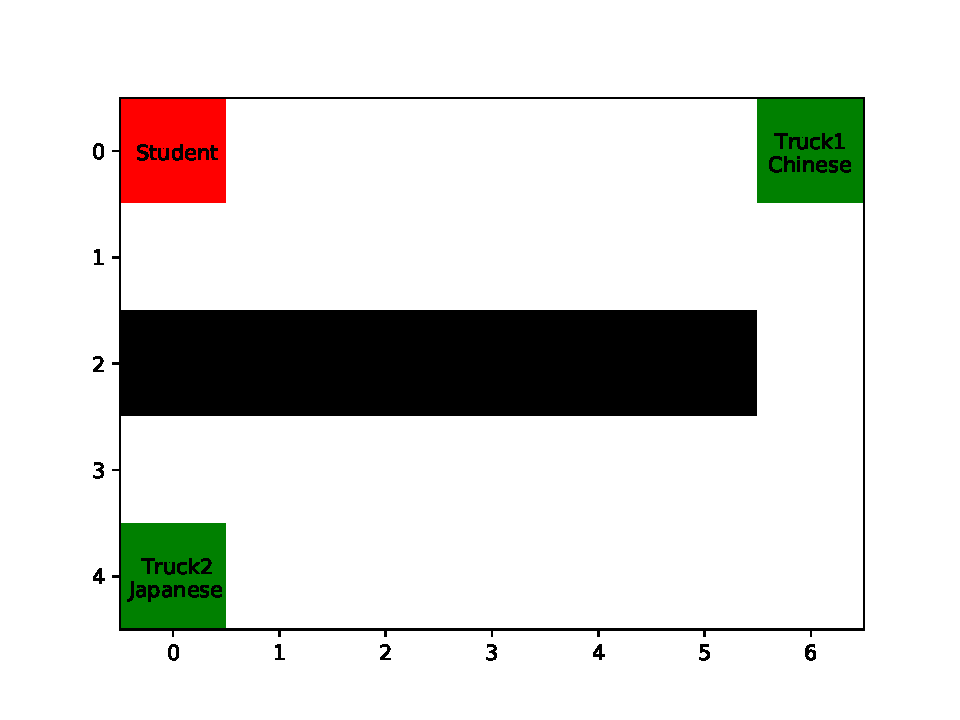
\includegraphics[]{./figure.pdf}
    \caption{本実験における環境}
    \label{fig:ex_env}
  \end{center}
\end{figure}

\par
図\ref{fig:ex_env}に本実験における環境の一例を示す.本実験には,本研究で作成したデータセットを利用した.本データセットには,屋台の組み合わせとその位置を含む環境設定と,その環境設定で考えられる学生の行動および発話が含まれる.30人の実験参加者に,本データセットで指定された環境設定と行動および発話を提示し,環境中の学生の信念と欲求をそれぞれ7段階で推定させた.またMIoMと,行動情報と発話情報の一方のみを基に心的状態を推定するUnimodal Inference of Mind(UIoM)により信念と欲求の推定を行った.MIoM(action + utterance),行動情報のみを基に心的状態を推定するUIoM(action),発話情報のみを基に心的状態を推定するUIoM(utterance)の3つのシステムによって,環境中の学生の信念と欲求をそれぞれ7段階で推定した.実験参加者によって得られた推定結果とMIoMおよびUIoM によって得られた推定結果を比較し相関係数を算出した.


\section{実験結果}

\begin{table}[htb]
  \begin{center}
  \caption{人間による推定と推定モデルの相関}
  \label{tab:cof}
  \begin{tabular}{lcc} \hline
    \multirow{2}{*}{モデル}&\multicolumn{2}{c}{相関}\\\cline{2-3}
    & \hspace{10pt} 信念 \hspace{10pt} & \hspace{10pt} 欲求 \hspace{10pt} \\ \hline
    UIoM(action)&0.124&0.419\\
    UIoM(utterance)&0.216&0.494\\
    MIoM(action + utterance)&\bf0.244&\bf0.549 \\\hline
  \end{tabular}
\end{center}
\end{table}


\par
表\ref{tab:cof}に,実験参加者による信念と欲求の推定結果とUIoM(action), UIoM(utterance)およびMIoMによる信念と欲求の推定結果との間の相関係数を示す.

\par
表\ref{tab:cof}より,MIoMは信念と欲求の推定の両方においてUIoM(action)およびUIoM(utterance)よりも強い相関を示した.また,いずれの推定システムにおいても欲求推定の相関が信念推定の相関よりも強いことがわかった.
